\documentclass{article}

\usepackage{fancyhdr}
\usepackage{extramarks}
\usepackage{amsmath}
\usepackage{amsthm}
\usepackage{amsfonts}
\usepackage{tikz}
\usepackage[plain]{algorithm}
\usepackage{algpseudocode}
\usepackage{xcolor}
\usepackage{enumitem}
\usepackage{amssymb}
\usepackage{todonotes}
\usepackage{mathtools}
\usepackage{wasysym}
\usepackage{cancel}

\usetikzlibrary{automata,positioning}

%
% Basic Document Settings
%

\topmargin=-0.45in
\evensidemargin=0in
\oddsidemargin=0in
\textwidth=6.5in
\textheight=9.0in
\headsep=0.25in

\linespread{1.1}

\pagestyle{fancy}
\lhead{\hmwkAuthorName}
\chead{\hmwkClass\ (\hmwkClassInstructor): \hmwkTitle}
\rhead{\firstxmark}
\lfoot{\lastxmark}
\cfoot{\thepage}

\renewcommand\headrulewidth{0.4pt}
\renewcommand\footrulewidth{0.4pt}

\setlength\parindent{0pt}

%
% Create Problem Sections
%

\newcommand{\enterProblemHeader}[1]{
    \nobreak\extramarks{}{Problem \arabic{#1} continued on next page\ldots}\nobreak{}
    \nobreak\extramarks{Problem \arabic{#1} (continued)}{Problem \arabic{#1} continued on next page\ldots}\nobreak{}
}

\newcommand{\exitProblemHeader}[1]{
    \nobreak\extramarks{Problem \arabic{#1} (continued)}{Problem \arabic{#1} continued on next page\ldots}\nobreak{}
    \stepcounter{#1}
    \nobreak\extramarks{Problem \arabic{#1}}{}\nobreak{}
}

\newcount\colveccount
\newcommand*\colvec[1]{
        \global\colveccount#1
        \begin{pmatrix}
        \colvecnext
}
\def\colvecnext#1{
        #1
        \global\advance\colveccount-1
        \ifnum\colveccount>0
                \\
                \expandafter\colvecnext
        \else
                \end{pmatrix}
        \fi
}

\setcounter{secnumdepth}{0}
\newcounter{partCounter}
\newcounter{homeworkProblemCounter}
\setcounter{homeworkProblemCounter}{1}
\nobreak\extramarks{Problem \arabic{homeworkProblemCounter}}{}\nobreak{}

%
% Homework Problem Environment
%
% This environment takes an optional argument. When given, it will adjust the
% problem counter. This is useful for when the problems given for your
% assignment aren't sequential. See the last 3 problems of this template for an
% example.
%
\newenvironment{homeworkProblem}[1][-1]{
    \ifnum#1>0
        \setcounter{homeworkProblemCounter}{#1}
    \fi
    \section{Problem \arabic{homeworkProblemCounter}}
    \setcounter{partCounter}{1}
    \enterProblemHeader{homeworkProblemCounter}
}{
    \exitProblemHeader{homeworkProblemCounter}
}

%
% Homework Details
%   - Title
%   - Due date
%   - Class
%   - Section/Time
%   - Instructor
%   - Author
%

\newcommand{\hmwkTitle}{Assignment 1}
\newcommand{\hmwkDueDate}{October 4, 2018}
\newcommand{\hmwkClass}{AFL}
\newcommand{\hmwkClassTime}{Fall Semester}
\newcommand{\hmwkClassInstructor}{Prof. Laura Pozzi}
\newcommand{\hmwkAuthorName}{\textbf{A. Romanelli}}

%
% Title Page
%

\title{
    \vspace{2in}
    \textmd{\textbf{\hmwkClass:\ \hmwkTitle}}\\
    \normalsize\vspace{0.1in}\small{Due\ on\ \hmwkDueDate\ at 11:55pm}\\
    \vspace{0.1in}\large{\textit{\hmwkClassInstructor}}
    \vspace{3in}
}

\author{\hmwkAuthorName}
\date{}

\renewcommand{\part}[1]{\textbf{\large Part \Alph{partCounter}}\stepcounter{partCounter}\\}

%
% Various Helper Commands
%

% Useful for algorithms
\newcommand{\alg}[1]{\textsc{\bfseries \footnotesize #1}}

% For derivatives
\newcommand{\deriv}[1]{\frac{\mathrm{d}}{\mathrm{d}x} (#1)}

% For partial derivatives
\newcommand{\pderiv}[2]{\frac{\partial}{\partial #1} (#2)}

% Integral dx
\newcommand{\dx}{\mathrm{d}x}

% Alias for the Solution section header
\newcommand{\solution}{\textbf{\large Solution}}

% Probability commands: Expectation, Variance, Covariance, Bias
\newcommand{\E}{\mathrm{E}}
\newcommand{\Var}{\mathrm{Var}}
\newcommand{\Cov}{\mathrm{Cov}}
\newcommand{\Bias}{\mathrm{Bias}}

\begin{document}

\maketitle

\pagebreak

\begin{homeworkProblem}
	Draw the FAs recognising the following Languages, over alphabet $\Sigma = \{0,1\}$:
\begin{center}
$$L1 = \{w | w \text{ has at most one 0 and at least two 1s }\}$$
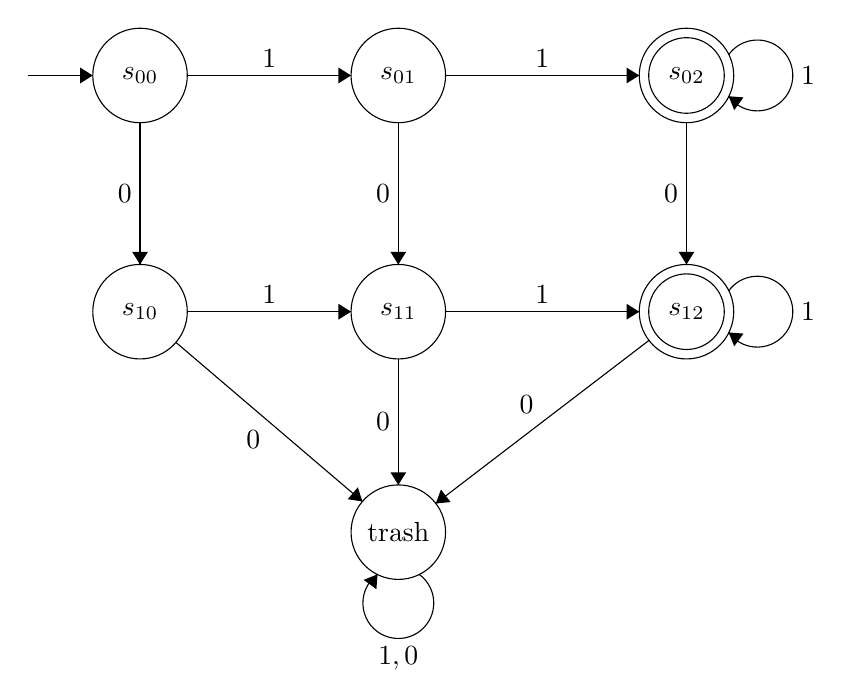
\begin{tikzpicture}[scale=0.2]
\tikzstyle{every node}+=[inner sep=0pt]
\draw [black] (11.9,-10.4) circle (3);
\draw (11.9,-10.4) node {$s_{00}$};
\draw [black] (28.3,-10.4) circle (3);
\draw (28.3,-10.4) node {$s_{01}$};
\draw [black] (28.3,-39.4) circle (3);
\draw (28.3,-39.4) node {trash};
\draw [black] (46.6,-10.4) circle (3);
\draw (46.6,-10.4) node {$s_{02}$};
\draw [black] (46.6,-10.4) circle (2.4);
\draw [black] (11.9,-25.4) circle (3);
\draw (11.9,-25.4) node {$s_{10}$};
\draw [black] (28.3,-25.4) circle (3);
\draw (28.3,-25.4) node {$s_{11}$};
\draw [black] (46.6,-25.4) circle (3);
\draw (46.6,-25.4) node {$s_{12}$};
\draw [black] (46.6,-25.4) circle (2.4);
\draw [black] (4.8,-10.4) -- (8.9,-10.4);
\fill [black] (8.9,-10.4) -- (8.1,-9.9) -- (8.1,-10.9);
\draw [black] (14.9,-10.4) -- (25.3,-10.4);
\fill [black] (25.3,-10.4) -- (24.5,-9.9) -- (24.5,-10.9);
\draw (20.1,-9.9) node [above] {$1$};
\draw [black] (31.3,-10.4) -- (43.6,-10.4);
\fill [black] (43.6,-10.4) -- (42.8,-9.9) -- (42.8,-10.9);
\draw (37.45,-9.9) node [above] {$1$};
\draw [black] (29.623,-42.08) arc (54:-234:2.25);
\draw (28.3,-46.65) node [below] {$1,0$};
\fill [black] (26.98,-42.08) -- (26.1,-42.43) -- (26.91,-43.02);
\draw [black] (11.9,-13.4) -- (11.9,-22.4);
\fill [black] (11.9,-22.4) -- (12.4,-21.6) -- (11.4,-21.6);
\draw (11.4,-17.9) node [left] {$0$};
\draw [black] (28.3,-13.4) -- (28.3,-22.4);
\fill [black] (28.3,-22.4) -- (28.8,-21.6) -- (27.8,-21.6);
\draw (27.8,-17.9) node [left] {$0$};
\draw [black] (14.9,-25.4) -- (25.3,-25.4);
\fill [black] (25.3,-25.4) -- (24.5,-24.9) -- (24.5,-25.9);
\draw (20.1,-24.9) node [above] {$1$};
\draw [black] (14.18,-27.35) -- (26.02,-37.45);
\fill [black] (26.02,-37.45) -- (25.73,-36.55) -- (25.09,-37.31);
\draw (19.09,-32.89) node [below] {$0$};
\draw [black] (28.3,-28.4) -- (28.3,-36.4);
\fill [black] (28.3,-36.4) -- (28.8,-35.6) -- (27.8,-35.6);
\draw (27.8,-32.4) node [left] {$0$};
\draw [black] (31.3,-25.4) -- (43.6,-25.4);
\fill [black] (43.6,-25.4) -- (42.8,-24.9) -- (42.8,-25.9);
\draw (37.45,-24.9) node [above] {$1$};
\draw [black] (46.6,-13.4) -- (46.6,-22.4);
\fill [black] (46.6,-22.4) -- (47.1,-21.6) -- (46.1,-21.6);
\draw (46.1,-17.9) node [left] {$0$};
\draw [black] (44.22,-27.22) -- (30.68,-37.58);
\fill [black] (30.68,-37.58) -- (31.62,-37.49) -- (31.01,-36.69);
\draw (36.45,-31.9) node [above] {$0$};
\draw [black] (49.28,-24.077) arc (144:-144:2.25);
\draw (53.85,-25.4) node [right] {$1$};
\fill [black] (49.28,-26.72) -- (49.63,-27.6) -- (50.22,-26.79);
\draw [black] (49.28,-9.077) arc (144:-144:2.25);
\draw (53.85,-10.4) node [right] {$1$};
\fill [black] (49.28,-11.72) -- (49.63,-12.6) -- (50.22,-11.79);
\end{tikzpicture}

$$L2 = \{w | w \text{ starts and ends with 1 and has even length }\}$$
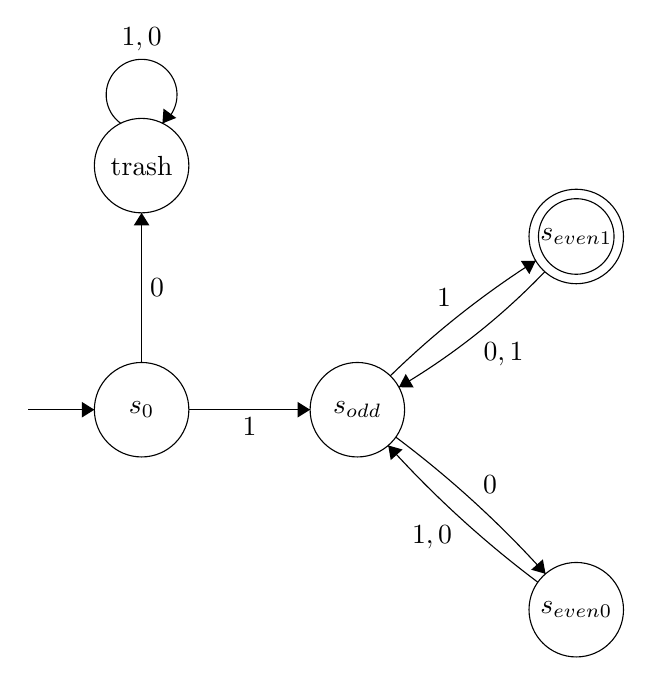
\begin{tikzpicture}[scale=0.2]
\tikzstyle{every node}+=[inner sep=0pt]
\draw [black] (18.5,-27.1) circle (3);
\draw (18.5,-27.1) node {$s_0$};
\draw [black] (32.2,-27.1) circle (3);
\draw (32.2,-27.1) node {$s_{odd}$};
\draw [black] (18.5,-11.6) circle (3);
\draw (18.5,-11.6) node {trash};
\draw [black] (46.1,-39.8) circle (3);
\draw (46.1,-39.8) node {$s_{even0}$};
\draw [black] (46.1,-16.1) circle (3);
\draw (46.1,-16.1) node {$s_{even1}$};
\draw [black] (46.1,-16.1) circle (2.4);
\draw [black] (11.3,-27.1) -- (15.5,-27.1);
\fill [black] (15.5,-27.1) -- (14.7,-26.6) -- (14.7,-27.6);
\draw [black] (21.5,-27.1) -- (29.2,-27.1);
\fill [black] (29.2,-27.1) -- (28.4,-26.6) -- (28.4,-27.6);
\draw (25.35,-27.6) node [below] {$1$};
\draw [black] (18.5,-24.1) -- (18.5,-14.6);
\fill [black] (18.5,-14.6) -- (18,-15.4) -- (19,-15.4);
\draw (19,-19.35) node [right] {$0$};
\draw [black] (34.642,-28.842) arc (53.19564:41.97041:65.808);
\fill [black] (44.15,-37.52) -- (43.98,-36.6) -- (43.24,-37.26);
\draw (40.62,-32.46) node [above] {$0$};
\draw [black] (34.292,-24.95) arc (134.27509:122.43876:57.11);
\fill [black] (43.53,-17.64) -- (42.58,-17.65) -- (43.12,-18.49);
\draw (37.71,-20.56) node [above] {$1$};
\draw [black] (43.661,-38.054) arc (-126.88444:-137.94951:66.751);
\fill [black] (34.16,-29.37) -- (34.32,-30.3) -- (35.07,-29.63);
\draw (36.94,-34.43) node [below] {$1,0$};
\draw [black] (17.177,-8.92) arc (234:-54:2.25);
\draw (18.5,-4.35) node [above] {$1,0$};
\fill [black] (19.82,-8.92) -- (20.7,-8.57) -- (19.89,-7.98);
\draw [black] (44.102,-18.337) arc (-43.76351:-59.52263:43.096);
\fill [black] (34.84,-25.67) -- (35.78,-25.69) -- (35.27,-24.83);
\draw (41.48,-22.82) node [below] {$0,1$};
\end{tikzpicture}
\end{center}
\newpage
\begin{center}
$$L3 = \{w | w \text{ has odd length or w has at most two 0s }\}$$
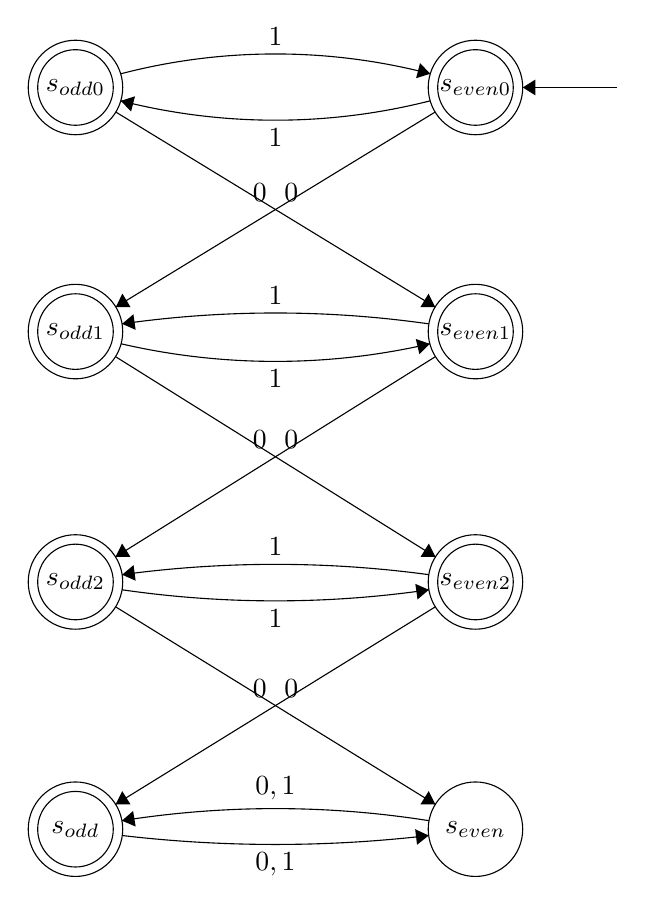
\begin{tikzpicture}[scale=0.2]
\tikzstyle{every node}+=[inner sep=0pt]
\draw [black] (30.5,-24.7) circle (3);
\draw (30.5,-24.7) node {$s_{odd1}$};
\draw [black] (30.5,-24.7) circle (2.4);
\draw [black] (55.9,-9.2) circle (3);
\draw (55.9,-9.2) node {$s_{even0}$};
\draw [black] (30.5,-9.2) circle (3);
\draw [black] (55.9,-9.2) circle (2.4);
\draw (30.5,-9.2) node {$s_{odd0}$};
\draw [black] (30.5,-9.2) circle (2.4);
\draw [black] (55.9,-24.7) circle (3);
\draw [black] (55.9,-24.7) circle (2.4);
\draw (55.9,-24.7) node {$s_{even1}$};
\draw [black] (55.9,-40.6) circle (3);
\draw [black] (55.9,-40.6) circle (2.4);
\draw (55.9,-40.6) node {$s_{even2}$};
\draw [black] (30.5,-40.6) circle (3);
\draw (30.5,-40.6) node {$s_{odd2}$};
\draw [black] (30.5,-40.6) circle (2.4);
\draw [black] (30.5,-56.3) circle (3);
\draw (30.5,-56.3) node {$s_{odd}$};
\draw [black] (30.5,-56.3) circle (2.4);
\draw [black] (55.9,-56.3) circle (3);
\draw (55.9,-56.3) node {$s_{even}$};
\draw [black] (33.04,-26.29) -- (53.36,-39.01);
\fill [black] (53.36,-39.01) -- (52.94,-38.16) -- (52.41,-39.01);
\draw (44.2,-32.15) node [above] {$0$};
\draw [black] (53.003,-25.476) arc (-76.97817:-103.02183:43.506);
\fill [black] (53,-25.48) -- (52.11,-25.17) -- (52.34,-26.14);
\draw (43.2,-27.09) node [below] {$1$};
\draw [black] (33.371,-8.332) arc (104.62381:75.37619:38.932);
\fill [black] (53.03,-8.33) -- (52.38,-7.65) -- (52.13,-8.61);
\draw (43.2,-6.57) node [above] {$1$};
\draw [black] (33.06,-10.76) -- (53.34,-23.14);
\fill [black] (53.34,-23.14) -- (52.92,-22.29) -- (52.4,-23.15);
\draw (44.2,-16.45) node [above] {$0$};
\draw [black] (52.942,-41.097) arc (-81.735:-98.265:67.767);
\fill [black] (52.94,-41.1) -- (52.08,-40.72) -- (52.22,-41.71);
\draw (43.2,-42.3) node [below] {$1$};
\draw [black] (53.36,-26.29) -- (33.04,-39.01);
\fill [black] (33.04,-39.01) -- (33.99,-39.01) -- (33.46,-38.16);
\draw (42.2,-32.15) node [above] {$0$};
\draw [black] (33.46,-24.211) arc (98.12525:81.87475:68.915);
\fill [black] (33.46,-24.21) -- (34.32,-24.59) -- (34.18,-23.6);
\draw (43.2,-23.02) node [above] {$1$};
\draw [black] (53.023,-10.048) arc (-75.72739:-104.27261:39.845);
\fill [black] (33.38,-10.05) -- (34.03,-10.73) -- (34.28,-9.76);
\draw (43.2,-11.78) node [below] {$1$};
\draw [black] (53.34,-10.76) -- (33.06,-23.14);
\fill [black] (33.06,-23.14) -- (34,-23.15) -- (33.48,-22.29);
\draw (42.2,-16.45) node [above] {$0$};
\draw [black] (53.35,-42.18) -- (33.05,-54.72);
\fill [black] (33.05,-54.72) -- (34,-54.73) -- (33.47,-53.88);
\draw (42.2,-47.95) node [above] {$0$};
\draw [black] (33.05,-42.18) -- (53.35,-54.72);
\fill [black] (53.35,-54.72) -- (52.93,-53.88) -- (52.4,-54.73);
\draw (44.2,-47.95) node [above] {$0$};
\draw [black] (33.451,-55.759) arc (99.00212:80.99788:62.308);
\fill [black] (33.45,-55.76) -- (34.32,-56.13) -- (34.16,-55.14);
\draw (43.2,-54.49) node [above] {$0,1$};
\draw [black] (52.927,-56.702) arc (-83.32647:-96.67353:83.702);
\fill [black] (52.93,-56.7) -- (52.07,-56.3) -- (52.19,-57.29);
\draw (43.2,-57.77) node [below] {$0,1$};
\draw [black] (33.464,-40.136) arc (97.71029:82.28971:72.57);
\fill [black] (33.46,-40.14) -- (34.32,-40.52) -- (34.19,-39.53);
\draw (43.2,-38.98) node [above] {$1$};
\draw [black] (64.9,-9.2) -- (58.9,-9.2);
\fill [black] (58.9,-9.2) -- (59.7,-9.7) -- (59.7,-8.7);
\end{tikzpicture}

$$L4 = \{w | w \text{ has at most length 4 and has as many 0s as 1s }\}$$
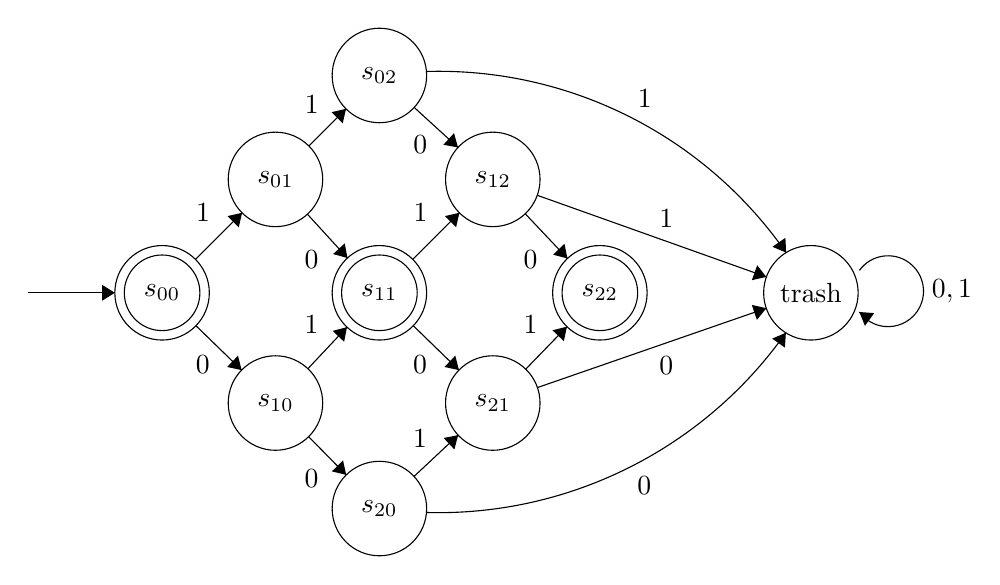
\begin{tikzpicture}[scale=0.2]
\tikzstyle{every node}+=[inner sep=0pt]
\draw [black] (9.5,-29.7) circle (3);
\draw (9.5,-29.7) node {$s_{00}$};
\draw [black] (9.5,-29.7) circle (2.4);
\draw [black] (16.7,-22.5) circle (3);
\draw (16.7,-22.5) node {$s_{01}$};
\draw [black] (16.7,-36.7) circle (3);
\draw (16.7,-36.7) node {$s_{10}$};
\draw [black] (23.3,-15.9) circle (3);
\draw (23.3,-15.9) node {$s_{02}$};
\draw [black] (23.3,-29.7) circle (3);
\draw (23.3,-29.7) node {$s_{11}$};
\draw [black] (23.3,-29.7) circle (2.4);
\draw [black] (23.3,-43.4) circle (3);
\draw (23.3,-43.4) node {$s_{20}$};
\draw [black] (30.5,-22.5) circle (3);
\draw (30.5,-22.5) node {$s_{12}$};
\draw [black] (30.5,-36.7) circle (3);
\draw (30.5,-36.7) node {$s_{21}$};
\draw [black] (37.3,-29.7) circle (3);
\draw (37.3,-29.7) node {$s_{22}$};
\draw [black] (37.3,-29.7) circle (2.4);
\draw [black] (50.7,-29.7) circle (3);
\draw (50.7,-29.7) node {trash};
\draw [black] (1,-29.7) -- (6.5,-29.7);
\draw [black] (62.28-8.5,-28.277) arc (144:-144:2.25);
\draw (66.85-8.5,-29.6) node [right] {$0,1$};
\fill [black] (62.28-8.5,-30.92) -- (62.63-8.5,-31.8) -- (63.22-8.5,-30.99);
\fill [black] (6.5,-29.7) -- (5.7,-29.2) -- (5.7,-30.2);
\draw [black] (11.62,-27.58) -- (14.58,-24.62);
\fill [black] (14.58,-24.62) -- (13.66,-24.83) -- (14.37,-25.54);
\draw (12.58,-24.62) node [left] {$1$};
\draw [black] (11.65,-31.79) -- (14.55,-34.61);
\fill [black] (14.55,-34.61) -- (14.32,-33.69) -- (13.63,-34.41);
\draw (12.08,-33.68) node [below] {$0$};
\draw [black] (18.82,-20.38) -- (21.18,-18.02);
\fill [black] (21.18,-18.02) -- (20.26,-18.23) -- (20.97,-18.94);
\draw (19.48,-17.72) node [left] {$1$};
\draw [black] (18.73,-24.71) -- (21.27,-27.49);
\fill [black] (21.27,-27.49) -- (21.1,-26.56) -- (20.36,-27.24);
\draw (19.46,-27.56) node [left] {$0$};
\draw [black] (18.76,-34.52) -- (21.24,-31.88);
\fill [black] (21.24,-31.88) -- (20.33,-32.12) -- (21.06,-32.81);
\draw (19.47,-31.73) node [left] {$1$};
\draw [black] (18.81,-38.84) -- (21.19,-41.26);
\fill [black] (21.19,-41.26) -- (20.99,-40.34) -- (20.28,-41.04);
\draw (19.47,-41.52) node [left] {$0$};
\draw [black] (25.51,-17.93) -- (28.29,-20.47);
\fill [black] (28.29,-20.47) -- (28.04,-19.56) -- (27.36,-20.3);
\draw (25.89,-19.69) node [below] {$0$};
\draw [black] (25.45,-31.79) -- (28.35,-34.61);
\fill [black] (28.35,-34.61) -- (28.12,-33.69) -- (27.43,-34.41);
\draw (25.88,-33.68) node [below] {$0$};
\draw [black] (25.5,-41.36) -- (28.3,-38.74);
\fill [black] (28.3,-38.74) -- (27.38,-38.92) -- (28.06,-39.65);
\draw (25.88,-39.56) node [above] {$1$};
\draw [black] (25.42,-27.58) -- (28.38,-24.62);
\fill [black] (28.38,-24.62) -- (27.46,-24.83) -- (28.17,-25.54);
\draw (26.38,-24.62) node [left] {$1$};
\draw [black] (32.56,-24.68) -- (35.24,-27.52);
\fill [black] (35.24,-27.52) -- (35.05,-26.59) -- (34.33,-27.28);
\draw (33.37,-27.57) node [left] {$0$};
\draw [black] (32.59,-34.55) -- (35.21,-31.85);
\fill [black] (35.21,-31.85) -- (34.29,-32.08) -- (35.01,-32.77);
\draw (33.37,-31.73) node [left] {$1$};
\draw [black] (33.33,-23.51) -- (47.87,-28.69);
\fill [black] (47.87,-28.69) -- (47.29,-27.95) -- (46.95,-28.9);
\draw (41.52,-25.57) node [above] {$1$};
\draw [black] (33.33,-35.72) -- (47.87,-30.68);
\fill [black] (47.87,-30.68) -- (46.95,-30.47) -- (47.27,-31.42);
\draw (41.51,-33.73) node [below] {$0$};
\draw [black] (49.108,-32.241) arc (-35.25325:-91.61664:27.012);
\fill [black] (49.11,-32.24) -- (48.24,-32.61) -- (49.05,-33.18);
\draw (40.12,-41.31) node [below] {$0$};
\draw [black] (26.288,-15.646) arc (91.66549:34.87033:26.884);
\fill [black] (49.13,-27.15) -- (49.08,-26.21) -- (48.26,-26.78);
\draw (40.15,-18) node [above] {$1$};
\end{tikzpicture}
\end{center}
\newpage
\begin{center}
$$L5 = \{w | w \text{ contains substring 11 and does not contain substring 00 }\}$$
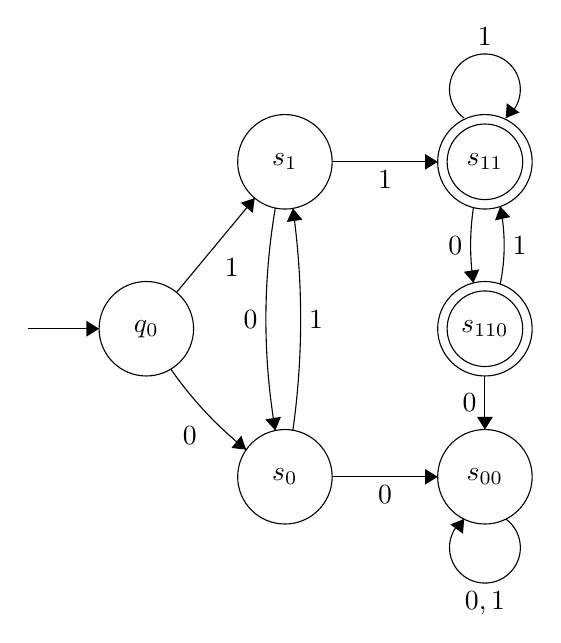
\begin{tikzpicture}[scale=0.2]
\tikzstyle{every node}+=[inner sep=0pt]
\draw [black] (17.1,-30.7) circle (3);
\draw (17.1,-30.7) node {$q_0$};
\draw [black] (25.9,-40.1) circle (3);
\draw (25.9,-40.1) node {$s_0$};
\draw [black] (38.6,-40.1) circle (3);
\draw (38.6,-40.1) node {$s_{00}$};
\draw [black] (25.9,-20.1) circle (3);
\draw (25.9,-20.1) node {$s_1$};
\draw [black] (38.6,-20.1) circle (3);
\draw (38.6,-20.1) node {$s_{11}$};
\draw [black] (38.6,-20.1) circle (2.4);
\draw [black] (38.6,-30.7) circle (3);
\draw [black] (46.077-8.8,-14.12-3.2) arc (234:-54:2.25);
\draw (47.4-8.8,-9.55-3.2) node [above] {$1$};
\fill [black] (48.72-8.8,-14.12-3.2) -- (49.6-8.8,-13.77-3.2) -- (48.79-8.8,-13.18-3.2);
\draw (38.6,-30.7) node {$s_{110}$};
\draw [black] (38.6,-30.7) circle (2.4);
\draw [black] (9.6,-30.7) -- (14.1,-30.7);
\fill [black] (14.1,-30.7) -- (13.3,-30.2) -- (13.3,-31.2);
\draw [black] (23.445,-38.38) arc (-128.56741:-145.20896:24.214);
\fill [black] (23.44,-38.38) -- (23.13,-37.49) -- (22.51,-38.27);
\draw (20.33,-37.46) node [left] {$0$};
\draw [black] (28.9,-40.1) -- (35.6,-40.1);
\fill [black] (35.6,-40.1) -- (34.8,-39.6) -- (34.8,-40.6);
\draw (32.25,-40.6) node [below] {$0$};
\draw [black] (39.923,-42.78) arc (54:-234:2.25);
\draw (38.6,-47.35) node [below] {$0,1$};
\fill [black] (37.28,-42.78) -- (36.4,-43.13) -- (37.21,-43.72);
\draw [black] (19.02,-28.39) -- (23.98,-22.41);
\fill [black] (23.98,-22.41) -- (23.09,-22.7) -- (23.86,-23.34);
\draw (22.05,-26.84) node [right] {$1$};
\draw [black] (28.9,-20.1) -- (35.6,-20.1);
\fill [black] (35.6,-20.1) -- (34.8,-19.6) -- (34.8,-20.6);
\draw (32.25,-20.6) node [below] {$1$};
\draw [black] (25.29,-37.163) arc (-170.31271:-189.68729:41.976);
\fill [black] (25.29,-37.16) -- (25.65,-36.29) -- (24.66,-36.46);
\draw (24.19,-30.1) node [left] {$0$};
\draw [black] (26.406,-23.057) arc (8.01773:-8.01773:50.498);
\fill [black] (26.41,-23.06) -- (26.02,-23.92) -- (27.01,-23.78);
\draw (27.4,-30.1) node [right] {$1$};
\draw [black] (37.872,-27.794) arc (-171.3417:-188.6583:15.904);
\fill [black] (37.87,-27.79) -- (38.25,-26.93) -- (37.26,-27.08);
\draw (37.19,-25.4) node [left] {$0$};
\draw [black] (38.6,-33.7) -- (38.6,-37.1);
\fill [black] (38.6,-37.1) -- (39.1,-36.3) -- (38.1,-36.3);
\draw (38.1,-35.4) node [left] {$0$};
\draw [black] (39.569,-22.931) arc (11.79139:-11.79139:12.083);
\fill [black] (39.57,-22.93) -- (39.24,-23.82) -- (40.22,-23.61);
\draw (40.32,-25.4) node [right] {$1$};
\end{tikzpicture}

$$L6 = \{w | w \text{ contains an even number of occurrences of substring 00 }\}$$
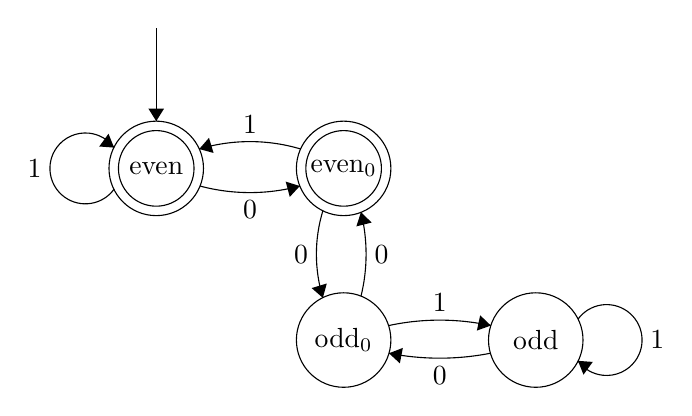
\begin{tikzpicture}[scale=0.2]
\tikzstyle{every node}+=[inner sep=0pt]
\draw [black] (19.2,-26.7) circle (3);
\draw (19.2,-26.7) node {even};
\draw [black] (19.2,-26.7) circle (2.4);
\draw [black] (31.1,-26.7) circle (3);
\draw (31.1,-26.7) node {$\text{even}_0$};
\draw [black] (31.1,-26.7) circle (2.4);
\draw [black] (31.1,-37.6) circle (3);
\draw (31.1,-37.6) node {$\text{odd}_0$};
\draw [black] (43.3,-37.6) circle (3);
\draw (43.3,-37.6) node {odd};
\draw [black] (28.325,-27.82) arc (-75.02254:-104.97746:12.285);
\fill [black] (28.32,-27.82) -- (27.42,-27.54) -- (27.68,-28.51);
\draw (25.15,-28.74) node [below] {$0$};
\draw [black] (40.423,-38.438) arc (-78.89845:-101.10155:16.741);
\fill [black] (33.98,-38.44) -- (34.67,-39.08) -- (34.86,-38.1);
\draw (37.2,-39.25) node [below] {$0$};
\draw [black] (45.98,-36.277) arc (144:-144:2.25);
\draw (50.55,-37.6) node [right] {$1$};
\fill [black] (45.98,-38.92) -- (46.33,-39.8) -- (46.92,-38.99);
\draw [black] (16.52,-28.023) arc (-36:-324:2.25);
\draw (11.95,-26.7) node [left] {$1$};
\fill [black] (16.52,-25.38) -- (16.17,-24.5) -- (15.58,-25.31);
\draw [black] (33.951,-36.683) arc (102.22433:77.77567:15.342);
\fill [black] (40.45,-36.68) -- (39.77,-36.03) -- (39.56,-37);
\draw (37.2,-35.84) node [above] {$1$};
\draw [black] (21.927,-25.47) arc (106.63727:73.36273:11.258);
\fill [black] (21.93,-25.47) -- (22.84,-25.72) -- (22.55,-24.76);
\draw (25.15,-24.5) node [above] {$1$};
\draw [black] (29.784,-34.918) arc (-162.96716:-197.03284:9.449);
\fill [black] (29.78,-34.92) -- (30.03,-34.01) -- (29.07,-34.3);
\draw (28.87,-32.15) node [left] {$0$};
\draw [black] (32.201,-29.481) arc (13.87375:-13.87375:11.131);
\fill [black] (32.2,-29.48) -- (31.91,-30.38) -- (32.88,-30.14);
\draw (33.03,-32.15) node [right] {$0$};
\draw [black] (19.2,-17.8) -- (19.2,-23.7);
\fill [black] (19.2,-23.7) -- (19.7,-22.9) -- (18.7,-22.9);
\end{tikzpicture}
\end{center}
\end{homeworkProblem}

\end{document}
